\documentclass{article}

% basics
\usepackage[utf8]{inputenc}
\usepackage[T1]{fontenc}
\usepackage{textcomp}
\usepackage{url}
\usepackage{hyperref}
\hypersetup{
    colorlinks,
    linkcolor={bb_g},
    citecolor={bb_g},
    urlcolor={bb_g}
}
\usepackage{graphicx}
\usepackage{float}
\usepackage{booktabs}
\usepackage{enumitem}
% \usepackage{parskip}
\usepackage{emptypage}
\usepackage{subcaption}
\usepackage{multicol}
\usepackage[usenames,dvipsnames]{xcolor}

% \usepackage{cmbright}

\usepackage{amsmath, amsfonts, mathtools, amsthm, amssymb}
\usepackage[left=1.5in,right=1.5in,top=1.5in,bottom=1.5in]{geometry}
\usepackage{mathrsfs}
\usepackage{cancel}
\usepackage{bm}
\newcommand\N{\ensuremath{\mathbb{N}}}
\newcommand\R{\ensuremath{\mathbb{R}}}
\newcommand\Z{\ensuremath{\mathbb{Z}}}
\renewcommand\O{\ensuremath{\emptyset}}
\newcommand\Q{\ensuremath{\mathbb{Q}}}
\newcommand\C{\ensuremath{\mathbb{C}}}
\renewcommand{\qedsymbol}{$\blacksquare$}
\DeclareMathOperator{\sgn}{sgn}
\usepackage{systeme}
\let\svlim\lim\def\lim{\svlim\limits}
\let\implies\Rightarrow
\let\impliedby\Leftarrow
\let\iff\Leftrightarrow
\let\epsilon\varepsilon
\usepackage{stmaryrd} % for \lightning
\newcommand\contra{\scalebox{1.1}{$\lightning$}}
\let\phi\varphi


% correct
\definecolor{correct}{HTML}{009900}
\newcommand\correct[2]{\ensuremath{\:}{\color{red}{#1}}\ensuremath{\to }{\color{correct}{#2}}\ensuremath{\:}}
\newcommand\green[1]{{\color{correct}{#1}}}


% Nord colors
\definecolor{d_0}{HTML}{2E3440}
\definecolor{d_1}{HTML}{3B4252}
\definecolor{d_2}{HTML}{434C5E}
\definecolor{d_3}{HTML}{4C566A}

\definecolor{w_0}{HTML}{D8DEE9}
\definecolor{w_1}{HTML}{E5E9F0}
\definecolor{w_2}{HTML}{ECEFF4}

\definecolor{b_ggg}{HTML}{8FBCBB}
\definecolor{b_gg}{HTML}{88C0D0}
\definecolor{b_g}{HTML}{81A1C1}
\definecolor{bb_g}{HTML}{5E81AC}

\definecolor{a_red}{HTML}{BF616A}
\definecolor{a_orange}{HTML}{D08770}
\definecolor{a_yellow}{HTML}{EBCB8B}
\definecolor{a_green}{HTML}{A3BE8C}
\definecolor{a_purple}{HTML}{B48EAD}


% Font
% \renewcommand{\familydefault}{\sfdefault}


% horizontal rule
\newcommand\hr{
    \noindent\rule[0.5ex]{\linewidth}{0.5pt}
}


% hide parts
\newcommand\hide[1]{}


% si unitx
\usepackage{siunitx}
\sisetup{locale = FR}
% \renewcommand\vec[1]{\mathbf{#1}}
\newcommand\mat[1]{\mathbf{#1}}


% tikz
\usepackage{tikz}
\usepackage{tikz-cd}
\usetikzlibrary{intersections, angles, quotes, calc, positioning}
\usetikzlibrary{arrows.meta}
\usepackage{pgfplots}
\pgfplotsset{compat=1.13}


\tikzset{
    force/.style={thick, {Circle[length=2pt]}-stealth, shorten <=-1pt}
}


% theorems
\makeatother
\usepackage{thmtools}
\usepackage[framemethod=TikZ]{mdframed}
\mdfsetup{skipabove=1em,skipbelow=0em}


\theoremstyle{definition}

\newcommand{\declaretheoremstylebox}[2]{
    \declaretheoremstyle[
        headfont=\bfseries\sffamily\color{#1}, bodyfont=\normalfont,
        mdframed={
            linewidth=2pt,
            rightline=false, topline=false, bottomline=false,
            linecolor=#1, backgroundcolor=#1!5
        }
    ]{thm#2box}    
}

\newcommand{\declaretheoremstyleline}[2]{
    \declaretheoremstyle[
        headfont=\bfseries\sffamily\color{#1}, bodyfont=\normalfont,
        mdframed={
            linewidth=2pt,
            rightline=false, topline=false, bottomline=false,
            linecolor=#1
        }
    ]{thm#2line}    
}

\declaretheoremstylebox{b_ggg}{green}
\declaretheoremstylebox{b_g}{blue}
\declaretheoremstylebox{a_red}{red}
\declaretheoremstylebox{a_orange}{orange}
\declaretheoremstylebox{a_yellow!60!a_orange}{yellow}

\declaretheoremstyleline{bb_g}{blue}
\declaretheoremstyleline{b_gg}{green}

\declaretheoremstyle[
    headfont=\bfseries\sffamily\color{a_red}, bodyfont=\normalfont,
    numbered=no,
    mdframed={
        linewidth=2pt,
        rightline=false, topline=false, bottomline=false,
        linecolor=a_red, backgroundcolor=a_red!1,
    },
    qed=\qedsymbol
]{thmproofbox}

\declaretheoremstyle[
    headfont=\bfseries\sffamily\color{b_g}, bodyfont=\normalfont,
    numbered=no,
    mdframed={
        linewidth=2pt,
        rightline=false, topline=false, bottomline=false,
        linecolor=b_g, backgroundcolor=b_g!1,
    },
]{thmexplanationbox}

% \declaretheoremstyle[headfont=\bfseries\sffamily, bodyfont=\normalfont, mdframed={ nobreak } ]{thmgreenbox}
% \declaretheoremstyle[headfont=\bfseries\sffamily, bodyfont=\normalfont, mdframed={ nobreak } ]{thmredbox}
% \declaretheoremstyle[headfont=\bfseries\sffamily, bodyfont=\normalfont]{thmbluebox}
% \declaretheoremstyle[headfont=\bfseries\sffamily, bodyfont=\normalfont]{thmblueline}
% \declaretheoremstyle[headfont=\bfseries\sffamily, bodyfont=\normalfont, numbered=no, mdframed={ rightline=false, topline=false, bottomline=false, }, qed=\qedsymbol ]{thmproofbox}
% \declaretheoremstyle[headfont=\bfseries\sffamily, bodyfont=\normalfont, numbered=no, mdframed={ nobreak, rightline=false, topline=false, bottomline=false } ]{thmexplanationbox}

\declaretheorem[style=thmgreenbox, name=Definition]{definition}
\declaretheorem[style=thmbluebox, numbered=no, name=Example]{example}
\declaretheorem[style=thmorangebox, name=Proposition]{proposition}
\declaretheorem[style=thmredbox, name=Theorem]{theorem}
\declaretheorem[style=thmyellowbox, name=Lemma]{lemma}
\declaretheorem[style=thmredbox, numbered=no, name=Corollary]{corollary}

\declaretheorem[style=thmproofbox, name=Proof]{replacementproof}
\renewenvironment{proof}[1][\proofname]{\vspace{-10pt}\begin{replacementproof}}{\end{replacementproof}}

\declaretheorem[style=thmexplanationbox, name=Proof]{tmpexplanation}
\newenvironment{explanation}[1][]{\vspace{-10pt}\begin{tmpexplanation}}{\end{tmpexplanation}}

\declaretheorem[style=thmgreenline, numbered=no, name=Remark]{remark}
\declaretheorem[style=thmblueline, numbered=no, name=Note]{note}

\newtheorem*{uovt}{UOVT}
\newtheorem*{notation}{Notation}
\newtheorem*{previouslyseen}{As previously seen}
\newtheorem*{problem}{Problem}
\newtheorem*{observe}{Observe}
\newtheorem*{property}{Property}
\newtheorem*{intuition}{Intuition}


\usepackage{etoolbox}
\AtEndEnvironment{vb}{\null\hfill$\diamond$}%
\AtEndEnvironment{intermezzo}{\null\hfill$\diamond$}%
% \AtEndEnvironment{opmerking}{\null\hfill$\diamond$}%

% http://tex.stackexchange.com/questions/22119/how-can-i-change-the-spacing-before-theorems-with-amsthm
\makeatletter
% \def\thm@space@setup{%
%   \thm@preskip=\parskip \thm@postskip=0pt
% }


\newcommand{\exercise}[1]{%
    \def\@exercise{#1}%
    \subsection*{Exercise #1}
}

\newcommand{\subexercise}[1]{%
    \subsubsection*{Exercise \@exercise.#1}
}


\usepackage{xifthen}

% Notes
\usepackage{marginnote}
\let\marginpar\marginnote

\def\testdateparts#1{\dateparts#1\relax}
\def\dateparts#1 #2 #3 #4 #5\relax{
    \marginpar{\small\textsf{\mbox{#1 #2 #3 #5}}}
}

\def\@lecture{}%
\newcommand{\lecture}[3]{
	\ifthenelse{\isempty{#3}}{%
		\def\@lecture{Lecture #1}%
	}{%
		\def\@lecture{Lecture #1: #3}%
	}%
	\section*{\@lecture}
	\marginpar{\small\textsf{\mbox{#2}}}
}


% \renewcommand\date[1]{\marginpar{#1}}


% fancy headers
\usepackage{fancyhdr}
\pagestyle{fancy}

% LE: left even
% RO: right odd
% CE, CO: center even, center odd
\fancyhead[LE, RO]{George C.}

\fancyhead[RO, LE]{\@lecture} % Right odd,  Left even
\fancyhead[RE, LO]{}          % Right even, Left odd
\fancyfoot[RO, LE]{\thepage}  % Right odd,  Left even
\fancyfoot[RE, LO]{}          % Right even, Left odd
\fancyfoot[C]{\leftmark}     % Center

\makeatother


% figure support
\usepackage{import}
\usepackage{xifthen}
\pdfminorversion=7
\usepackage{pdfpages}
\usepackage{transparent}
\newcommand{\incfig}[1]{%
    \def\svgwidth{\columnwidth}
    \import{./figures/}{#1.pdf_tex}
}

% %http://tex.stackexchange.com/questions/76273/multiple-pdfs-with-page-group-included-in-a-single-page-warning
\pdfsuppresswarningpagegroup=1

\setcounter{section}{-1}

\title{Math 1540: HW1}

\begin{document}

\maketitle
\emph{Book Problems:}
\begin{enumerate}
    \item[55.]
    If \((f,g) = h \neq 1\), then there must exist an extension field of \(F\), \(E\), which contains a root of \(h\) which is common between \(f\) and \(g\) since \((f,g) = h\)

    Else, \((f,g) = 1\), then there exists no field \(E\) containing both \(F\) and a common root of \(f(x)\) and \(g(x)\) since \((\exists a, b \in F)(af + bg = 1)\) implies \(f\) and \(g\) share no roots (\(a(x)f(x)+ b(x)g(x) = 1 \neq 0\) for all \(x\)).   

    \item[56.] 
    \begin{enumerate}
    \item[(i)]
    Let \(f(x) = a_0 + a_1 x \ldots + a_n x^n \) then:
    \begin{eqnarray*}
        (f(x))^p = (a_0 + a_1 x \ldots + a_n x^n)^p \\
        = a_0^p + a_1^p (x)^p \ldots + a_n^p (x^n)^p 
    \end{eqnarray*}
    Because of Fermat's Little Theorem \(a^p \equiv a \pmod p\):
    \begin{eqnarray*}
        = a_0 + a_1 (x)^p \ldots + a_n (x^n)^p \\
        = a_0 + a_1 (x^p) \ldots + a_n (x^p)^n \\
        = f(x^p) 
    \end{eqnarray*}
    
    \item[(ii)] If we replace \(\mathbb{Z}_p\) with an infinite field, \(F\), of characteristic \(p\) we can be no longer sure that Fermat's Little Theorem holds for all \(a_i\) in \(f(x) = a_0 + a_1 x \ldots + a_n x^n \). \(x^p - x\) only has \(p\) roots, and they are only the elements \(\mathbb{Z}_p \subset F\). \(a_i\) could be in \(F\) and not \(\mathbb{Z}_p\), so we are left will a less strong result: \((f(x))^p = a_0^p + a_1^p x^p \ldots + a_n^p (x^p)^n = g(x^p)\)  
    \end{enumerate}
    \item[61.] Let's factor \(x^8 - x\) in \(\mathbb{Z}_2\) 
    \begin{eqnarray*}
        x^8 - x \\
        x(x^7 - 1) \\
        x(x-1)(x^6 + x^5 + x^4 + x^3 + x^2 + x + 1)
    \end{eqnarray*}
    Since we are in \(\mathbb{Z}_2\), \(3 = 1\) and we can factor it further:  
    \begin{eqnarray*}
        x(x-1)(x^6 + x^5 + x^4 + 3x^3 + x^2 + x + 1) \\
        x(x-1)(x^3+x+1)(x^3+x^2+1)  
    \end{eqnarray*}
    Now we can use either \(x^3+x+1\) or \(x^3+x^2+1\). I will use \(x^3+x+1\).
    \(\mathbb{Z}_2/(x^3+x+1) \cong \mathbb{F}_8\) so our elements will be \(1, x, x + 1, x^2, x^2 + 1, x^2 + x, x^2 + x + 1\)
    
    Therefore, our addition table will look like:
    \begin{align*}
        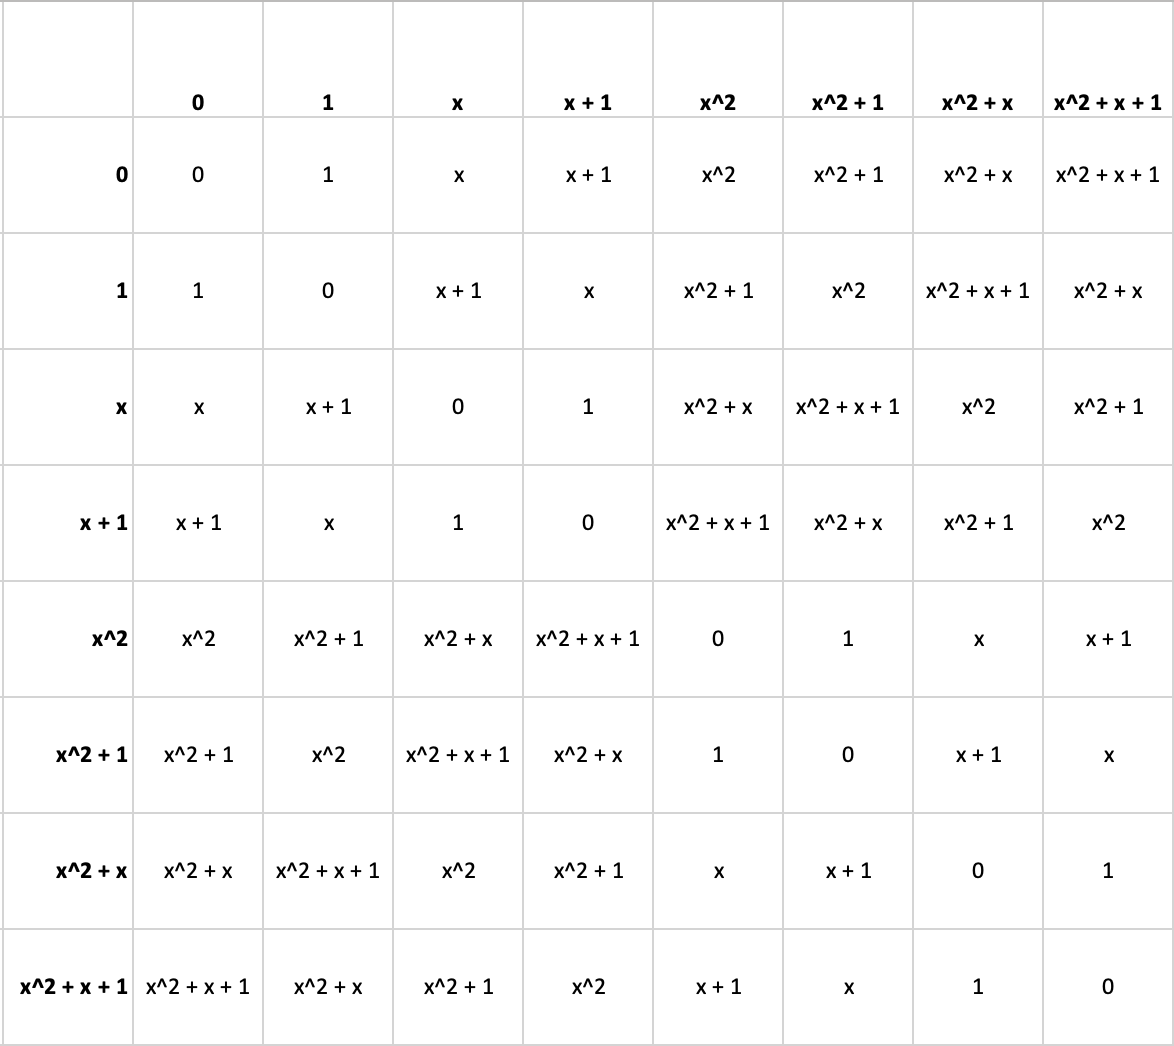
\includegraphics[scale=.45]{F8+.png} 
    \end{align*}
    
    And, our multiplication table will look like
    
    \begin{align*}
        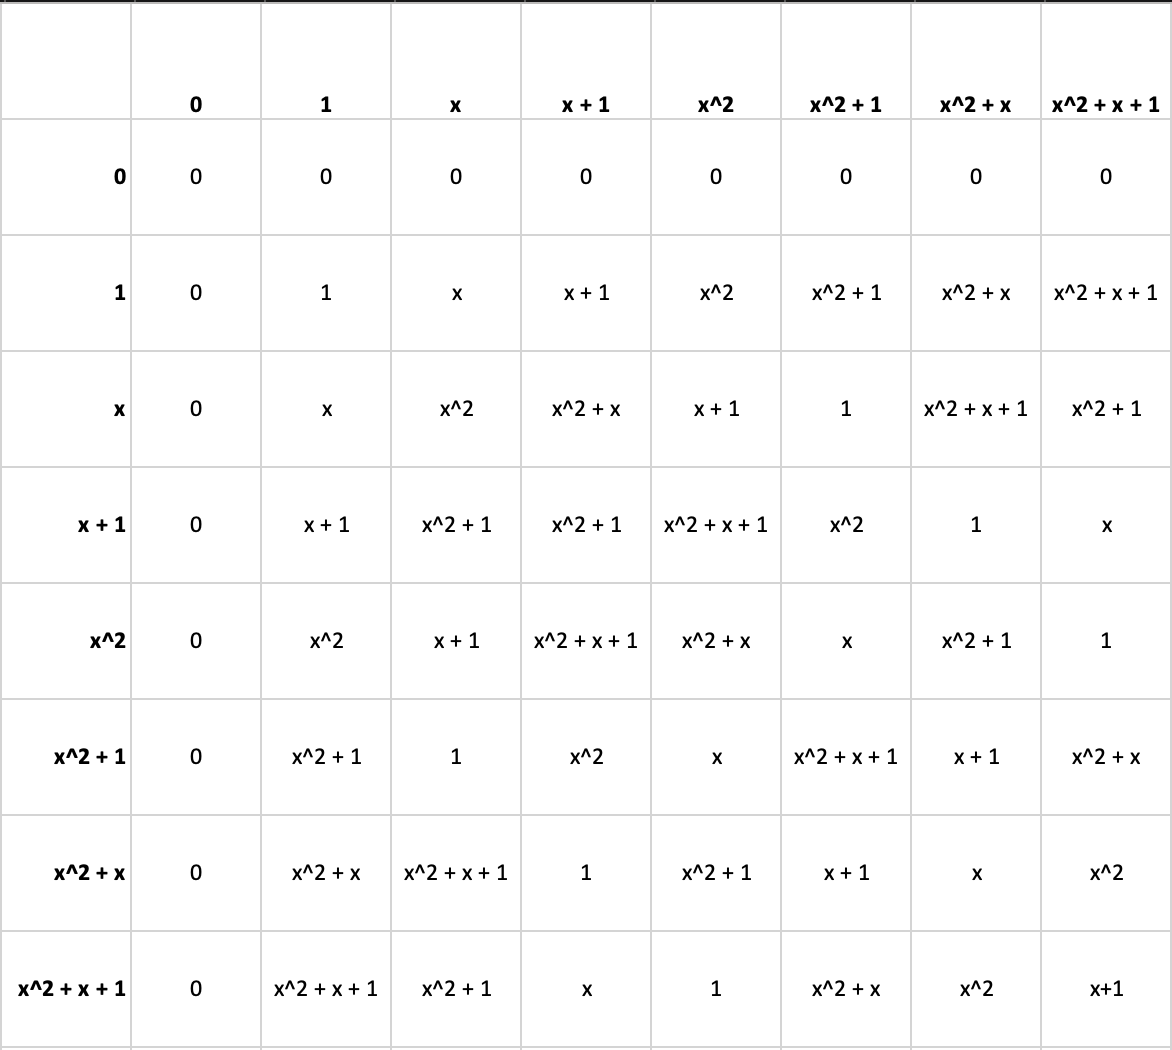
\includegraphics[scale=.45]{F8*.png}
    \end{align*}

    (Sorry for the non LaTeX, the tables were giving a lot of trouble)

    \item[62.] If \(\mathbb{F}_4\) was isomorphic to a subfield of \(\mathbb{F}_8\), there would have to be a field extension of \(\mathbb{F}_4\) to \(\mathbb{F}_8\), a \(\mathbb{F}_4\) vector space of dimension \(n\); however this would imply \(\exists n \in \mathbb{Z}, 4^n = 8\), which is not possible, so it is not possible that \(\mathbb{F}_4\) is isomorphic to a subfield of \(\mathbb{F}_8\).
\end{enumerate}

\emph{Given Problems:}
\begin{enumerate}
    \item[1.] \(f\) has no repeated roots if and only if \((f,f^\prime) = 1\) is equivalent to \(f\) has repeated roots if and only if \((f,f^\prime) \neq 1\)
    
    Assume \(f(x)\) has repeated roots then \(f(x) = (x-\alpha)^k g(x)\) where \((\alpha)\) is a repeated root. If \(f(x) = (x-\alpha)^k g(x)\), then \(f^\prime(x) = k(x-\alpha)^{k-1}g(x) + (x-\alpha)g^\prime (x) = (x-\alpha)(k (x-\alpha)^{k-2} g(x) + g^\prime (x))\). Therefore, \((x-\alpha) | (f, f^\prime) \implies (f, f^\prime) \neq 1\)
    
    Assume \((f,f^\prime) \neq 1\) then \((f,f^\prime)\) is a non-constant polynomial, \(h(x)\). Then \(f = h(x)g_1(x)\) and \(f^\prime = h(x)g_2(x)\) Therefore, \(f\) and \(f^\prime\) share roots of \(h(x)\) and so \(f\) has repeated roots. 

    \item[2.] 
    Let \(f = h f^\prime\) and \(g = h g^\prime \) where \(h, f^\prime, g^\prime \in F[x]\) and \(f^\prime\) and \(g^\prime\) are relatively prime.   

    Then \(\exists a,b \in F\) s.t:
    \begin{eqnarray*}
        af^\prime  + bg^\prime = 1 
    \end{eqnarray*}
    which is equivalent to
    \begin{eqnarray*}
        h(af^\prime  + bg^\prime) = h(1) \\
        h af^\prime  + h bg^\prime = h \\
        af + bg = h 
    \end{eqnarray*}

    Since \(\exists a,b \in E\)
    \[
        af^\prime  + bg^\prime = 1
    \]
    in \(E\), this implies
    \[
        af + bg = h
    \]

    Therefore, \((f,g)_F = (f,g)_E = h\) 

    % Let \(h = (f, g)_F\) and \(j = (f, g)_E\)

    % \(h \in E[x]\) so \(h | f,g \implies h|j\)

    % \((\exists a, b \in F[x])(a f + b g = h)\) and \(a, b \in E[x]\) so \(h \in (j) \implies j | h\)
    
    % Since \(j | h\) and \(h | j\), \(h = j\)  

    \item[3.] Eisenstein's Criterion says that if you have a polynomial $f(x) = a_{n}x^{n} + a_{n-1}x^{n-1} + \hdots + a_{1}x + a_{0}$, and a prime $p$ dividing each $a_{i}$ for $0 \leq i < n$, but $p$ doesn't divide $a_{n}$ and $p^{2}$ doesn't divide $a_{0}$, then $f(x)$ is irreducible in $\Q[x]$. For \(f(x) = x^n - m\), the conditions to meet the criterion are simplified to \(p | m \wedge p \nmid 1 \wedge p^2 \nmid m\) since \(a_0 = m\) and \(a_n = 1\). Let \(m\) be expressed as a prime factorization \(p_1\ldots p_n\). By the definition of square free \((\forall p \in {p_1\ldots p_n})(p^2 \nmid m)\). Therefore, \((\forall p \in {p_1\ldots p_n})(p | m \wedge p \nmid 1 \wedge p^2 \nmid m)\).

    \item[4.] Let \(f(x) = x^4 + 6x^3 + 12x^2 + 6x + 1\) Let's apply a coordinate transformation to \(f(x)\). Since a coordinate transformation does not change whether a polynomial is irreducible, we can pick a clever coordinate transformation to make the problem simpler. Since there are multiple terms with positive coefficients that are multiples of \(6\) making a coordinate transformation of \(x-1\) might be a good choice. \(f(x -1) = 2 - 4x + 2x^3 + x^4\) Now we can use Eisenstein's Criterion more easily. Recall Eisenstein's Criterion says that if you have a polynomial $g(x) = a_{n}x^{n} + a_{n-1}x^{n-1} + \hdots + a_{1}x + a_{0}$, and a prime $p$ dividing each $a_{i}$ for $0 \leq i < n$, but $p$ doesn't divide $a_{n}$ and $p^{2}$ doesn't divide $a_{0}$, then $g(x)$ is irreducible in $\Q[x]$. Using Eisenstein's criterion on \(f(x - 1)\) , we can see that a prime \(p = 2\) divides each $a_{i}$ for $0 \leq i < n$ (\(2 | 2,-4, 2\)), $p = 2$ doesn't divide $a_{n} = 1$, and $p^{2} = 4$ doesn't divide $a_{0} = 2$; therefore, $f(x - 1)$ is irreducible in $\Q[x]$ and so $f(x)$ is irreducible in $\Q[x]$. 
\end{enumerate}

\end{document}